Esta seção apresenta o protocolo experimental e os resultados produzidos a partir deste protocolo.

\begin{figure}
    \caption{Elementos estruturante em tons de cinza alvos 7x7.}
    \centering
    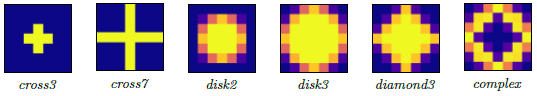
\includegraphics[scale=0.8]{images/ElementosEstruturantes}
    \label{fig:elementos-estruturantes}
\end{figure}

\subsection{Protocolo experimental}
\label{subsec:protocolo-experimental}

A seguir, foi avaliada a capacidade das camadas $\mathcal{L}$Morph e $\mathcal{S}$Morph propostas de aprenderem um elemento estruturante alvo e os resultados obtidos comparado com camada de \emph{PConv}.
Para tanto, as operações de dilatação $\oplus$, erosão $\ominus$, fechamento $\bullet$ e abertura $\circ$ foram aplicadas para todos os 60000 digitos do conjunto de dados MNIST, com elementos esturantes alvos apresentados na figura~\ref{fig:elementos-estruturantes}.
Mas precisamente, em se tratando das operaçãoes de dilatação e erosão, construi-se uma rede composta de apenas uma única camada seguida de um escalar/coeficiente linear de convolução 1x1x1 para re-escalar os valores de saída dentro do intervalor das imagens alvo.
Quanto as operações de fechamento e abertura, foram utilizados uma rede composta de duas camadas, respectivamente, dilatação e erosão e, erosão e dilatação.
Valendo salientar que, devidos as limitações já apresentadas, ambas as redes \emph{PConv} e $\mathcal{L}$Morph também tiveram que ser re-escaladas em [1, 2] antes de passarem por qualquer camada morfológica.
Todas as redes foram treinadas com um \emph{batch size} de 32, otimizado pela perda erro médio quadrático(MSE) com o otimizador Adam utilizando uma taxa de aprenizado $\eta = 0.01$.
A taxa de aprendizado do otimizador foi programada para decrementar por um fator de 10 quando o plato da perda se manter por 5 épocas consecutivas.
A convergence é tida como alcançada quando o plato da perda se estabilizar por 10 épocas consecutivas.

Para os filtros da camada \emph{PConv}, foram-se iniciados os filtros com $1$ e $p = 0$.
Para $\mathcal{L}$Morph, os filtros foram iniciados com distribuição normal dobrada com desvio padrão $\sigma = 0.01$ e $p = 0$.
Camadas $\mathcal{S}$Morph, com seus filtros inicializados com uma distribuição normal centrada com o desvio padrão $\sigma = 0.01$ e $\alpha = 0$.

Objetivando avaliar a desempenho das redes morfológicas para todos os cenários (isto é, para cada elemento estruturante operando $\oplus, \ominus, \bullet, \circ$), computou-se entre o filtro aprendido na convergência e o filtro alvo, a raiz do erro médio quadrático (RMSE).
Computando a perda na convergência bem como os valores dos parâmetros $p$ ou $\alpha$ úteis, também, como critério quanatitativo.

\begin{figure}
    \caption{Elementos estruturantes aprendidos (com seus correspondentes $p$ e $\alpha$ na convergência) pelas camadas \emph{PConv}, $\mathcal{L}$Morph e $\mathcal{S}$Morph em tarefas de dilatação $\oplus$ e erosão $\ominus$.}
    \centering
    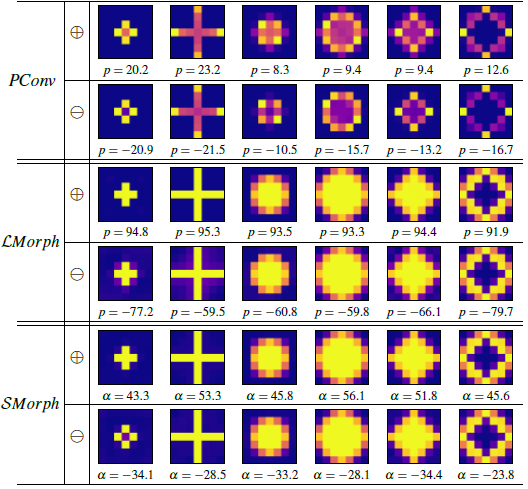
\includegraphics[scale=0.9]{images/ElementosEstrurantesAprendidos1}
    \label{fig:elementos-estruturantes-aprendidos-1}
\end{figure}

\begin{table}
    \caption{Perda do MSE na convergência e o RMSE entre o elemento estruturante aprendido apresentado pela figura~\ref{fig:elementos-estruturantes-aprendidos-1} e o alvo para as camadas \emph{PConv}, $\mathcal{L}$Morph e $\mathcal{S}$Morph nas tarefas de diltação $\oplus$ e erosão $\ominus$. Os melhores (menores) resultados estão em negrito.}
    \centering
    \label{tab:elementos-estruturantes-aprendidos-1}
    \resizebox{\textwidth}{!}{
        \begin{tabular}{*{10}l}
            &                            &      & \emph{cross3} & \emph{cross7} & \emph{disk2}  & \emph{disk3}  & \emph{diamond3} & \emph{complex} & \\
            \hline
            \multirow{4}{*}{\emph{PConv}}      & \multirow{2}{*}{$\oplus$}  & LOSS & 0.5           & 0.8           & 5.1           & 6.4           & 6.8 & 3.3 & $\times 10^{-4}$\\
            &                            & RMSE & 0.41          & 1.42          & 2.22          & 3.09          & 2.80            & 2.38           &                                          \\
            \cline{3-10}
            & \multirow{2}{*}{$\ominus$} & LOSS & 2.4           & 0.62          & 13            & 2.6           & 5.2             & 1.2            & $\times 10^{-5}$                         \\
            &                            & RMSE & 0.82          & 1.55          & 2.82          & 3.77          & 3.63            & 2.76           &                                          \\
            \hline
            \hline
            \multirow{4}{*}{$\mathcal{L}$Morh} & \multirow{2}{*}{$\oplus$}  & LOSS & 0.84          & 1.2           & 0.78          & 1.2 & 1.2 & 2.1 & $\times 10^{-5}$\\
            &                            & RMSE & \textbf{0.02} & \textbf{0.0 } & \textbf{0.02} & \textbf{0.05} & \textbf{0.01}   & \textbf{0.48} & \\
            \cline{3-10}
            & \multirow{2}{*}{$\ominus$} & LOSS & 1.1           & \textbf{0.37} & 1.3           & \textbf{0.37} & 0.58            & \textbf{1.1} & $\times 10^{-6}$ \\
            &                            & RMSE & \textbf{0.44} & 0.63          & 0.37          & 0.29          & 0.38            & \textbf{0.48}  &                                          \\
            \hline
            \hline
            \multirow{4}{*}{$\mathcal{S}$Morh} & \multirow{2}{*}{$\oplus$}  & LOSS & \textbf{1.8}  & \textbf{4.0} & \textbf{2.5} & \textbf{4.9} & \textbf{3.9} & \textbf{1.7} & $\times$ \textbf{10\textsuperscript{-7}} \\
            &                            & RMSE & 0.10          & 0.13          & 0.08          & 0.06          & 0.09            & 0.51           &                                          \\
            \cline{3-10}
            & \multirow{2}{*}{$\ominus$} & LOSS & 210           & 4.1           & \textbf{0.8}  & 4.1           & \textbf{4.3}    & \textbf{9.5} & $\times$ \textbf{10\textsuperscript{-7}} \\
            &                            & RMSE & 0.78          & \textbf{0.15} & \textbf{0.09} & \textbf{0.05} & \textbf{0.09}   & 0.51           &                                          \\
            \hline
        \end{tabular}
    }
\end{table}


\begin{figure}
    \caption{Elementos estruturantes aprendidos (com seus correspondentes $p$ e $\alpha$ na convergência) pelas camadas \emph{PConv}, $\mathcal{L}$Morph e $\mathcal{S}$Morph em tarefas de fechamento $\bullet$ e abertura $\circ$.}
    \centering
    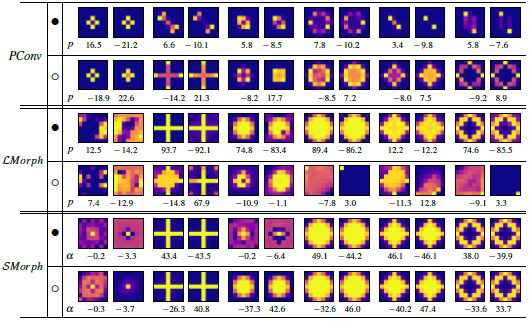
\includegraphics[scale=0.9]{images/ElementosEstrurantesAprendidos2}
    \label{fig:elementos-estruturantes-aprendidos-2}
\end{figure}

\begin{table}
    \caption{Perda do MSE na convergência e o RMSE entre o elemento estruturante aprendido apresentado pela figura~\ref{fig:elementos-estruturantes-aprendidos-2} e o alvo para as camadas \emph{PConv}, $\mathcal{L}$Morph e $\mathcal{S}$Morph nas tarefas de fechamento $\bullet$ e abertura $\circ$. Os melhores (menores) resultados estão em negrito.}
    \centering
    \label{tab:elementos-estruturantes-aprendidos-2}
    \resizebox{\textwidth}{!}{
        \begin{tabular}{*{10}l}
            &                            &      & \emph{cross3}                 & \emph{cross7}                 & \emph{disk2}                  & \emph{disk3}                  & \emph{diamond3}               & \emph{complex} & \\
            \hline
            \multirow{4}{*}{\emph{PConv}}      & \multirow{2}{*}{$\bullet$} & LOSS & 0.09                          & 5.1                           & 1.7                           & 1.0                           & 5.4 & 4.9 & $\times 10^{-e}$\\
            &                            & RMSE & \textbf{0.83} | \textbf{0.81} & 3.94 | 3.97                   & 2.82 | 3.07                   & 4.44 | 4.64                   & 4.34 | 4.61 & 3.68 | 3.65 &                  \\
            \cline{3-10}
            & \multirow{2}{*}{$\circ$}   & LOSS & \textbf{0.86}                 & 0.76                          & 4.8                           & 3.9                           & 4.4                           & 2.3                           & $\times 10^{-4}$                         \\
            &                            & RMSE & \textbf{0.91} | \textbf{0.32} & 1.45 | 0.87                   & 2.70 | 2.49                   & 3.10 | 2.52                   & 3.15 | 2.43 & 2.10 | 2.08 &                  \\
            \hline
            \hline
            \multirow{4}{*}{$\mathcal{L}$Morh} & \multirow{2}{*}{$\bullet$} & LOSS & \textbf{0.5}                  & 0.13 & \textbf{2.0} & 0.18 & 6.2 & 0.14 & $\times 10^{-4}$\\
            &                            & RMSE & 3.58 | 5.12                   & \textbf{0.01} | 0.63          & \textbf{0.14} | \textbf{1.16} & \textbf{0.07} | 0.40 & 0.75 | 0.95 & \textbf{0.47} | 0.99 & \\
            \cline{3-10}
            & \multirow{2}{*}{$\circ$}   & LOSS & 8.7                           & 36                            & 2.0                           & 2.7                           & 4.6                           & 2.5                           & $\times 10^{-3}$                         \\
            &                            & RMSE & 3.17 | 4.74                   & 2.90 | 1.20                   & 1.99 | 1.61                   & 2.81 | 5.56                   & 1.66 | 3.54                   & 2.72 | 3.98                   &                                          \\
            \hline
            \hline
            \multirow{4}{*}{$\mathcal{S}$Morh} & \multirow{2}{*}{$\bullet$} & LOSS & 1700                          & \textbf{0.31} & 4400 & \textbf{0.42} & \textbf{0.37} & \textbf{0.17} & $\times$ \textbf{10\textsuperscript{-6}} \\
            &                            & RMSE & 2.10 | 3.59                   & 0.14 | 0.08                   & 2.78 | 3.68                   & 0.08 | 0.01                   & 0.08 | 0.10                   & 0.52 | 0.52                   &                                          \\
            \cline{3-10}
            & \multirow{2}{*}{$\circ$}   & LOSS & 4700                          & \textbf{0.14}                 & \textbf{0.22}                 & \textbf{0.25}                 & \textbf{0.24} & \textbf{0.09} & $\times$ \textbf{10\textsuperscript{-6}} \\
            &                            & RMSE & 3.40 | 1.63                   & \textbf{0.18} | \textbf{0.02} & \textbf{0.05} | \textbf{0.01} & \textbf{0.02} | \textbf{0.02} & \textbf{0.02} | \textbf{0.01}  & \textbf{0.51} | \textbf{0.52} & \\
            \hline

        \end{tabular}
    }
\end{table}

\subsection{Resultados obtidos}
\label{subsec:resultados-obtidos}

Todas as redes (\emph{PConv}, $\mathcal{L}$Morph, $\mathcal{S}$Morph) conseguiram, por meio dos sinais dos parâmetros aplicar operações morfológicas corretamente.
A partir da magnetude observada na convergência, também é possível constatar que as operações aplicadas pelas redes podem ser consideradas dilatação e erosão (e, não simplesmente uma pseudo-dilatação ou pseudo-erosão).
Entretanto, enquanto o formato dos elementos estruturantes aprendidos pela camada de \emph{PConv} sofre um efeito de concavidade, as camadas $\mathcal{L}$Morph e $\mathcal{S}$Morph precisamente recuperam seus elementos estruturantes alvos.
Confirmados pelos valores de RMSE calculados entre o elemento estruturante alcançado durante a convergência e o elemento estruturante alvo apresentado na figura~\ref{fig:elementos-estruturantes}.
Mais precisamente, a operação de dilatação atingiu valores de RMSE mais baixos nas camadas de $\mathcal{L}$Morph e a erosão, com valores baixos nas camadas de $\mathcal{S}$Morph.
A figura \{\emph{incluir a figura 5}\} apresenta os elementos estruturantes aprendidos nas camadas de \emph{PConv}, $\mathcal{L}$Morph e $\mathcal{S}$Morph para as operações de abertura e fechamento.
Mas, desta vez, englobando duas camadas com filtros independentes um do outro.
A rede $\mathcal{L}$Morph foi capaz de aprender corretamente a operação e forma para os grandes elementos estruturantes nas operações de fechamento, com exceção do \emph{cross3} e \emph{disk2}.
Mas o contra-desempenho contantentemente falho percebido nas operações de abertura não até agora não foram explicados.
Tendo a rede $\mathcal{S}$Morph apresentado resultados pouco satisfatórios a pequenos elementos estruturantes para ambas operações de fechamento e abertura, é visto bons resultados nos maiores.
Nos casos extremos de pequenos elementos estruturantes alvos poderia vir da escala/convolução de coeficiênte linear 1x1x1, que super-compensa erros durante a fase de aprendizagem.
Poderia não ter aprendido corretamente todos os filtros por trás da escala//convolução de coeficiênte linear 1x1x1 com parametros $p$ e $\alpha$ não convergindo sobre os domínios de sinais corretos.


